\section*{Bugs}
\addcontentsline{toc}{section}{Bugs}

\subsection*{Canto Bug}
\addcontentsline{toc}{subsection}{Canto Bug}
\begin{itemize}
\item In most fire emblem games, if you move a mounted unit with a longer path than necessary, then the game calculates your remaining movement based off of the shortest path required to get to your destination (as opposed to what you actually drew). Three Houses does not do this for you - if you draw a path longer than necessary, then you will end up having less remaining movement to canto with (or even be unable to canto at all).
\item This is important to call out because many strats rely on taking advantage of the remaining movement for your mounted units (particularly part 2). If you overlook this bug and accidentally draw a longer path, you'll likely end up messing up your strategy and thus have to waste time undoing that with divine pulse - worst-case scenario, this mistake will end your turn, and you'l have to sit through several level ups or even some deaths.
\item This bug can be occasionally exploited to save a little bit of time though - if you don't need to canto nor your entire movement range, then it can be advantageous to intentionally draw a suboptimal path that uses up all of that unit's movement - this is because after an action, if a mounted unit is prompted to canto, they will have an annoying 1-second long animation of posing in place. This is called out in the "Map Movement" segment above. Note that this is extremely situational, and is rarely useful - you're usually better off dismounting.
\end{itemize}

\begin{figure}[h]
\centerline{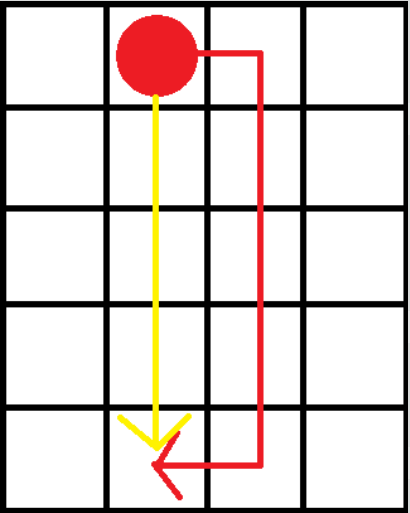
\includegraphics[scale=.4]{./General Information/canto.png}}
\caption{Pegasus Knights are mounted and have 6 movement. In other Fire Emblem games, if a Pegasus Knight takes the red path then an action, then that unit can canto up to 2 tiles, because the game calculated that only 4 tiles were actually needed to reach that tile (yellow path). Unfortunately, Three Houses will not calculate this for you, and instead, will just not let you canto, because it calculates the remaining movement as if you used up all 6 tiles. If a Wyvern Rider or Cavalier with 7 move took the same red path and an action, they would have 1 move left to canto in 3H, and 3 move left in all other fire emblem games.}
\end{figure}

\subsection*{The Door}
\addcontentsline{toc}{subsection}{The Door}
\begin{itemize}
\item In the early game, when controlling \Byleth\ in the Monastery for the first time, you have to talk to the three House Lords. Past \Edelgard\ is a door that seemingly randomly doesn't open for 9-10 seconds, which can cause a large early timeloss.
\item You can set up the game so that this doesn't happen by doing the following steps:
\begin{enumerate}
	\item Set up a save file in the Officer's Academy - Monastery for the first time, during the first quest
	\item Before every batch of attemps, load the save file, reset, and then start the run
	\item You don't necessarily need to open the save file before every attempt, but you'll probably want to load it again if you reset past Chapter 5 or so.
\end{enumerate}
\end{itemize}